\documentclass{article}

\usepackage[utf8]{inputenc}
\usepackage[LGR, T1]{fontenc}
\usepackage[greek]{babel} % This automatically transcribes letters. Use \textlatin to escape it
\usepackage{amsmath, amsfonts,amssymb}
\usepackage{amsthm}
\usepackage{alphabeta}

\usepackage{graphicx}
\graphicspath{ {../output/} }


% To make custom snippets, Ctrl+shift+P --> Preferences: Configure User Snippets -> latex (or latex.json)
\DeclareMathOperator{\E}{\mathrm{E}}
\DeclareMathOperator{\V}{\mathrm{V}}
\DeclareMathOperator{\Var}{\mathrm{Var}}
\DeclareMathOperator{\Cov}{\mathrm{Cov}}
\DeclareMathOperator{\se}{\mathrm{se}}
% \DeclareMathOperator{\tr}{\mathrm{tr}}
\DeclareMathOperator{\rank}{\mathrm{rank}}
\newcommand{\inner}[2]{\left\langle #1 \mathrel{,} #2 \right\rangle}
\newcommand{\norm}[1]{\left\| #1 \right\|}
\newcommand{\T}[1]{{#1}^{\top}}  % alternatively, use {#1}^{\intercal} or {#1}'
% Using this for lines in matrices: https://tex.stackexchange.com/a/12914/256497
\newcommand*{\vertbar}{\rule[-1ex]{0.5pt}{2.5ex}}
\newcommand*{\horzbar}{\rule[.5ex]{2.5ex}{0.5pt}}
\newcommand{\SSE}{\mathrm{SSE}}
\newcommand{\SSR}{\mathrm{SSR}}
\newcommand{\SST}{\mathrm{SST}}
\newcommand{\MSE}{\mathrm{MSE}}
\newcommand{\hb}{\hat{\beta}}
% \newcommand{\Sxx}{S_{xx}}
% \newcommand{\Sxy}{S_{xy}}
% \newcommand{\Syy}{S_{yy}}
\newcommand{\ve}[1]{\boldsymbol{#1}}


\renewcommand{\thesection}{\Alph{section}}
\renewcommand{\thesubsection}{\thesection.\roman{subsection}}
\newtheorem{exercise}{Άσκηση}[section]


\title{\textbf{Στατιστική Μοντελοποίηση} \\ Πρώτη Σειρά ασκήσεων}
\author{Κωνσταντίνος Παπαδάκης\\\scriptsize{ΕΔΕΜΜ 03400149}}
\date{\today}


\begin{document}

\begin{titlepage}
    \maketitle
\end{titlepage}

\section{Μέρος}

\textbf{Δείξτε ότι για το \underline{απλό γραμμικό μοντέλο} \(\E[Y] = β_0 + β_1 X\) ισχύουν τα ακόλουθα:}


%%%%%%%%%%%%%%%% EXERCISE 1 %%%%%%%%%%%%%%%%
\begin{exercise}
    \(R^2 = r_{xy}^2\), \(R^2\) ο συντελεστής προσδιορισμού, \(r_{xy}\) ο δειγματικός συντελεστής συσχέτισης (\textlatin{Pearson}) των \(x\) και \(y\) παρατηρήσεων.
\end{exercise}
\begin{proof}
    Ισχύει ότι
    \begin{align}
        \hb_1 &= \frac{S_{xy}}{S_{xx}}\\
        \hb_0 &= \bar{y} - \hb_1 \bar{x}\\
        r_{xy} &= \frac{S_{xy}}{\sqrt{S_{xx} S_{yy}}}\\
        \SSR &= \hb_1^2 S_{xx}\\
        \SST &= S_{yy}
    \end{align}
    Έτσι έχουμε
    \begin{equation*}
    \begin{split}
        R^2 &= \frac{\SSR}{\SST}\\
            &= \frac{\hb_1^2 S_{xx}}{S_{yy}}\\
            &= \frac{S_{xy}^2}{S_{xx}^2} \frac{S_{xx}}{S_{yy}}\\
            &= \frac{S_{xy}^2}{S_{xx} S_{yy}}\\
            &= r_{xy}^2
    \end{split}
    \end{equation*}
\end{proof}


%%%%%%%%%%%%%%%% EXERCISE 2 %%%%%%%%%%%%%%%%
\begin{exercise}
    \begin{equation*}
        \sum_{i=1}^n y_i = \sum_{i=1}^n \hat{y}_i
    \end{equation*}
\end{exercise}
\begin{proof}
    Για να αποδείξουμε το αποτέλεσμα θα ορίσουμε κάποιους πίνακες και θα αποδείξουμε μερικές ιδιότητές τους.

    Ορίζουμε
    \begin{align*}
        Ι := \begin{pmatrix}
            1 & & \\
             & \ddots & \\
             & & 1
        \end{pmatrix}\\
        J := \frac{1}{n} \begin{pmatrix}
            1 & \dots & 1\\
            \vdots & \ddots & \vdots\\
            1 & \dots & 1
        \end{pmatrix}\\
        H := X (\T{X} X)^{-1} \T{X}
    \end{align*}
    % όπου οι \(I\) και \(J\) είναι διάστασης \(n \times n\) και ο \(H\) είναι διάστασης \(p \times p\).
    οπου όλοι τους είναι διάστασης \(n \times n\).

    Και οι τρεις αυτοί πίνακες είναι \emph{προβολές} αφού είναι εύκολο να δει κανείς πως είναι \emph{συμμετρικοί} και \emph{ταυτοδύναμοι}. Οι υπόχωροι που αντιστοιχούν σε αυτές τις προβολές είναι οι εξής:
    \begin{itemize}
        \item Για τον \(I\) είναι όλος χώρος στον οποίον ορίζεται.
        \item Για τον \(J\) ειναι ο χώρος που παράγεται από το \(\ve{1} := \T{\begin{pmatrix} 1 & \dots & 1 \end{pmatrix}}\).
            Αυτό ισχύει αφού \(\rank J = 1\) και \( J \ve{1} = \ve{1} \) 
        \item Για τον \(H\) είναι ο χώρος που παράγεται από της στήλες του \(X\) (μία εξ αυτών η \(\ve{1}\)). Aυτό ισχύει αφού
        \begin{equation*}
            \begin{pmatrix} HX^{(1)} & \dots & HX^{(p)} \end{pmatrix} = HX = X = \begin{pmatrix} X^{(1)} & \dots & X^{(p)} \end{pmatrix}
        \end{equation*}
        και \(\rank H \leq \rank X = p\)
    \end{itemize}

    Παρατηρούμε ότι η \(J\) είναι \emph{υποπροβολή} της \(H\) αφού o χώρος που παράγεται από το \(\ve{1}\) είναι υπόχωρος του στηλοχώρου του \(X\).
    Αυτό σημαίνει ότι \(HJ = JH = J\).
    Σημείωση ότι από αυτό προκύπτει ότι η προβολή \(I - J\) αναλύεται στις κάθετες μεταξύ τους προβολές \(H - J\) και \(I - H\) από όπου προκύπτει η ισότητα \(\SSE = \SSR + \SST\).

    Θα χρησιμοποίησουμε τον συμβολισμό \(\inner{\ve{x}}{\ve{y}}\) για το ευκλείδιο εσωτερικό γινόμενο.

    Το ζητούμενο αποτέλεσμα είναι ισοδύναμο με το \(\sum (y_i - \hat{y}_i) = 0\), το οποίο ισχύει αφού
    \begin{equation*}
    \begin{split}
        \sum (y_i - \hat{y}_i) &= \inner{(I - H) \ve{y}}{\ve{1}}\\
        &= \inner{\ve{y}}{\T{(I - H)} \ve{1}}\\
        &= \inner{\ve{y}}{(I - H) \ve{1}}\\
        &= \inner{\ve{y}}{\ve{1} - H \ve{1}}\\
        &= \inner{\ve{y}}{\ve{1} - \ve{1}}\\
        &= \ve{0}
    \end{split}
    \end{equation*}
\end{proof}


%%%%%%%%%%%%%%%% EXERCISE 3 %%%%%%%%%%%%%%%%
\begin{exercise} \label{ex3}
    \begin{equation*}
        \Cov(\bar{y}, \hb_1) = 0
    \end{equation*}
\end{exercise}
\begin{proof}
    Έχουμε,
    \begin{equation*}
    \begin{split}
        \Cov(\bar{y}, \hb_1) &= \Cov(\hb_0 + \hb_1 \bar{x}, \hb_1)\\
        &= \Cov(\hb_0, \hb_1) + \Cov(\hb_1, \hb_1) \bar{x}
    \end{split}
    \end{equation*}
    
Θα βρούμε τις σχετικές συνδιακυμάνσεις από τον πίνακα διακύμανσης του \(\hb\), δηλαδή τον \( \V(\hb) = \sigma^2 (\T{X} X)^{-1} \)
Έχουμε,
\begin{equation*}
    \T{X} X  =  \begin{pmatrix}
                    \horzbar & \ve{1} & \horzbar\\
                    \horzbar & \ve{x} & \horzbar
                \end{pmatrix}
                \begin{pmatrix}
                    \vertbar & \vertbar\\
                    \ve{1} & \ve{x}\\
                    \vertbar & \vertbar
                \end{pmatrix}
              = \begin{pmatrix}
                    \inner{\ve{1}}{\ve{1}} & \inner{\ve{1}}{\ve{x}}\\
                    \inner{\ve{x}}{\ve{1}} & \inner{\ve{x}}{\ve{x}}
                \end{pmatrix}
              = \begin{pmatrix}
                    n & n \bar{x}\\
                    n \bar{x} & \norm{\ve{x}}^2
                \end{pmatrix}
\end{equation*}

Άρα,
\begin{equation*}
    (\T{X} X)^{-1} = \frac{1}{n\norm{\ve{x}}^2 - n^2 \bar{x}} 
                     \begin{pmatrix}
                         \norm{\ve{x}}^2 & -n\bar{x}\\
                         -n\bar{x} & n
                     \end{pmatrix}
\end{equation*}

Συνεπώς,
\begin{align*}
    \Cov(\bar{y}, \hb_1) &= \Cov(\hb_0, \hb_1) + \Cov(\hb_1, \hb_1) \bar{x}\\
    &\propto \left( -n\bar{x} \right) + \left( n \right) \bar{x}\\
    &= 0\\
    \implies \Cov(\bar{y}, \hb_1) &= 0
\end{align*}
\end{proof}


%%%%%%%%%%%%%%%% EXERCISE 4 %%%%%%%%%%%%%%%%
\begin{exercise}
    \begin{equation*}
        \sum y_i \hat{y}_i = \sum \hat{y}_i^2
    \end{equation*}
\end{exercise}
\begin{proof}
    Το ζητούμενο αποτέλεσμα είναι ισοδύναμο με το \(\sum \hat{y}_i (y_i - \hat{y}_i) = 0\).

    Έχουμε,
    \begin{equation*}
    \begin{split}
        \sum \hat{y}_i (y_i - \hat{y}_i) &= \inner{\ve{\hat{y}}}{\ve{y} - \ve{\hat{y}}}\\
        &= \inner{H \ve{y}}{(I-H) \ve{y}}\\
        &= \inner{\ve{y}}{\T{H}(I - H)\ve{y}}\\
        &= \inner{\ve{y}}{H(I - H)\ve{y}}\\
        &= \inner{\ve{y}}{\ve{0}}\\
        &= 0
    \end{split}
    \end{equation*}
\end{proof}


%%%%%%%%%%%%%%%% EXERCISE 5 %%%%%%%%%%%%%%%%
\begin{exercise}
    \begin{equation*}
        \sum \left( y_i - \hat{y}_i \right) \left(\hat{y}_i - \bar{y}\right) = 0
    \end{equation*}
\end{exercise}
\begin{proof}
    \begin{equation*}
    \begin{split}
        \sum \left( y_i - \hat{y}_i \right) \left(\hat{y}_i - \bar{y}\right) &= \inner{\ve{y} - H\ve{y}}{H\ve{y} - J\ve{y}}\\
        &= \inner{(I - H) \ve{y}}{(H - J) \ve{y}}\\
        &\stackrel{*}{=} 0
    \end{split}
    \end{equation*}

    Όπου η τελευταία (*) ισότητα ισχύει αφού η \(H - J\) είναι η υποπροβολή της H (προβολή στις στήλες του \(X\) πλην της \(\ve{1}\)),
    και η \(I - H\) είναι η προβολή στον κάθετο χώρο που προβάλει η \(H\) (δηλαδή στον \(\mathrm{Im}(X)^{\bot}\)).
    
    Ποιο αναλυτικά,
    \begin{equation*}
        \left( I - H \right) \left( H - J \right) =
        H - J - H^2 + HJ =
        H - J - H + J =
        0
    \end{equation*}
\end{proof}


%%%%%%%%%%%%%%%% EXERCISE 6 %%%%%%%%%%%%%%%%
\begin{exercise}
    \begin{equation*}
        \frac{\hb_1}{\se(\hb_1)} = \frac{r_{xy} \sqrt{n-2}}{\sqrt{1 - r_{xy}^2}}
    \end{equation*}
\end{exercise}
\begin{proof}

    Από την \ref{ex3} ξέρουμε ότι
    \begin{equation*}
    \begin{split}
        \V[\hb_1] &= \sigma^2 \frac{1}{n \norm{\ve{x}}^2 - n^2 \bar{x}^2}\\
        &=\frac{\sigma^2}{\norm{\ve{x}}^2 - n \bar{x}^2}
    \end{split}
    \end{equation*}
    
    Θα χρειαστούμε το παρακάτω αποτέλεσμα,
    \begin{equation*} 
    \begin{split}
        S_{xx} &= \sum \left( x_i - \bar{x} \right)^2\\
        &= \norm{(I - J)\ve{x}}^2\\
        &= \T{\ve{x}} \T{(I - J)} (I - J) \ve{x}\\
        &= \T{\ve{x}} (I - J) \ve{x}\\
        &= \norm{\ve{x}}^2 - \T{\ve{x}} \left( J x \right)\\
        &= \norm{\ve{x}}^2 - \T{\ve{x}} (\bar{x} \ve{1})\\
        &= \norm{\ve{x}}^2 - \bar{x} (\T{\ve{x}} \ve{1})\\
        &= \norm{\ve{x}}^2 - \bar{x} (n \bar{x})\\
        &= \norm{\ve{x}}^2 - n \bar{x}^2\\
    \end{split}
    \end{equation*}

    Έτσι καταλήγουμε στο ότι
    \begin{equation*}
        \V[\hb_1] = \frac{\sigma^2}{S_{xx}}
    \end{equation*}

    απο το οποίο παίρνουμε
    \begin{equation*} 
        \se(\hb_1)^2 = \frac{s^2}{S_{xx}}
    \end{equation*}

    Έχουμε,
    \begin{equation*} \tag{*} \label{eqn}
    \begin{split}
        &r_{xy}^2 = R^2 = 1 - \frac{\SSE}{\SST}\\
        \implies& 1 - r_{xy}^2 = \frac{\SSE}{\SST}\\
        \implies& \SST \left( 1 - r_{xy}^2 \right) = \SSE\\
    \end{split}
    \end{equation*}

    Χρησμοποιόντας τις ισότητες \(s^2 = \frac{\SSE}{n-2}\) και \(\SST = S_{yy}\), τότε από την \eqref{eqn} συμπεραίνουμε ότι
    \begin{equation*}
        s^2 = \frac{1}{n-2} S_{yy} \left( 1 - r_{xy}^2 \right)
    \end{equation*}

    Χρησμοποιόντας την παραπάνω έκφραση έχουμε
    \begin{equation*}
        \begin{split}
            \left( \frac{\hb_1}{\se(\hb_1)} \right)^2 &= \frac{\hb_1^2}{\frac{s^2}{S_{xx}}}\\
            &= \frac{S_{xy}^2 / S_{xx}^2}{\frac{1}{S_{xx}}  \frac{1}{n-2} S_{yy} \left( 1 - r_{xy}^2 \right)}\\
            &= \frac{S_{xy}^2 (n-2)}{S_{xx} S_{yy} \left( 1 - r_{xy}^{2} \right)}\\
            &= \frac{r_{xy}^2 (n-2)}{1 - r_{xy}^2}
        \end{split}
    \end{equation*}

    Συνεπώς,
    \begin{equation*}
        \frac{\hb_1}{\se(\hb_1)} = \frac{r_{xy} \sqrt{n-2}}{\sqrt{1 - r_{xy}^2}}
    \end{equation*}
\end{proof}

%%%%%%%%%%%%%%%%%%%%%%%%%%%%%%%%%%%%%%%%%%%%%%%%%%%%%%
%%%%%%%%%%%%%%%%%%%%%%%%%%%%%%%%%%%%%%%%%%%%%%%%%%%%%%
%%%%%%%%%%%%%%%%%%%%%%%%%%%%%%%%%%%%%%%%%%%%%%%%%%%%%%
%%%%%%%%%%%%%%%%%%%%%%%%%%%%%%%%%%%%%%%%%%%%%%%%%%%%%%
%%%%%%%%%%%%%%%%%%%%%%%%%%%%%%%%%%%%%%%%%%%%%%%%%%%%%%

\section{Μέρος}
Τα δεδομένα στο αρχείο \textlatin{cholesterol.txt} αφορούν επίπεδα ολικής χοληστερόλης
\textlatin{(mg/ml)} 24 ασθενών (\(y\)) και την ηλικία τους (\(x\)).

\subsection{}
\subsubsection*{Εκφώνηση}
Να κατασκευαστεί ένα διάγραμμα διασποράς μεταξύ των δύο μεταβλητών \(y\) και
\(x\) και να προσαρμοστεί το μοντέλο \(\E[y] = \hb_0 + \hb_1 x\).
\subsubsection*{Απάντηση}
Στο Σχήμα \ref{fig:part-b-scatter} βλέπουμε το σχετικό διάγραμμα 
\begin{figure}[h]
    \centering
    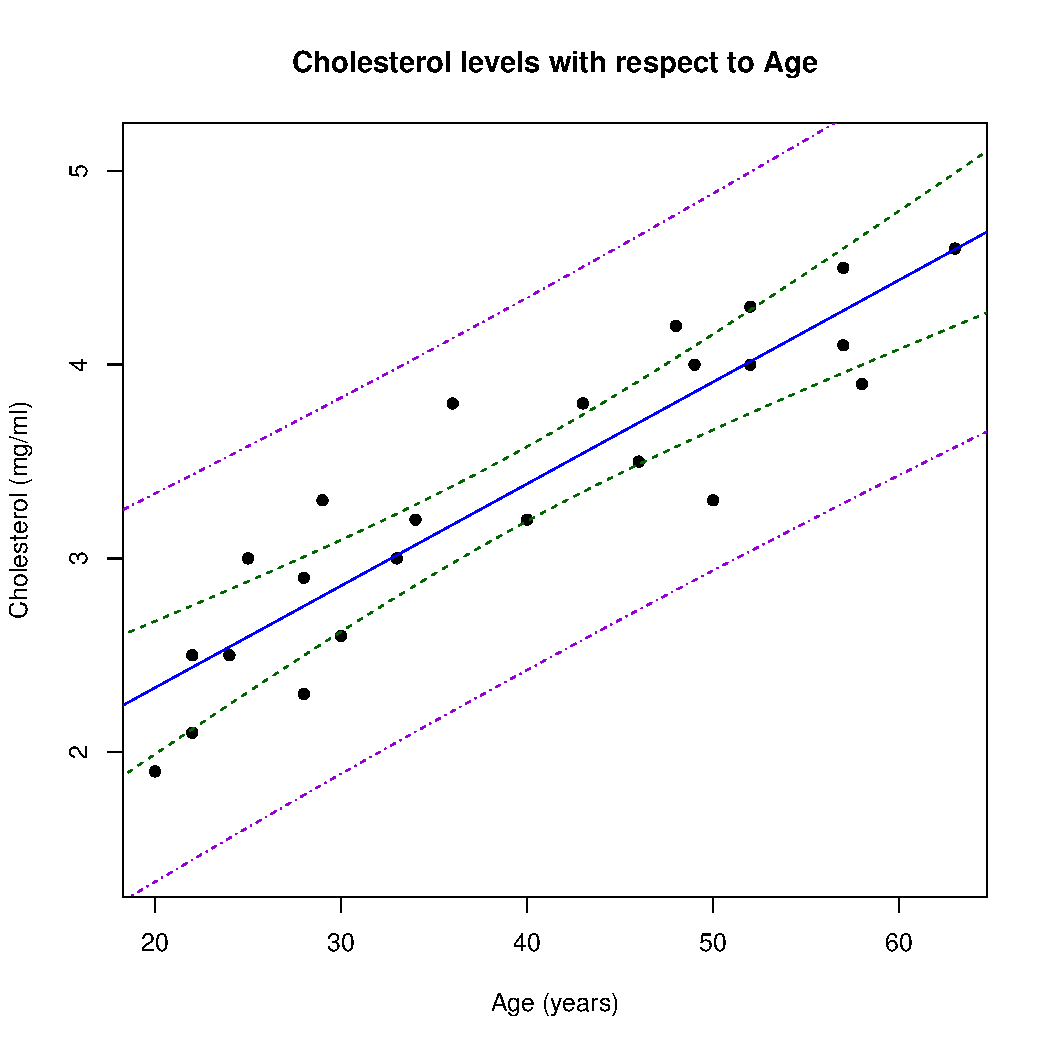
\includegraphics[width=1.0\textwidth]{part-b-scatter.pdf}
    \caption{Διάγραμμα διασποράς για τα επίπεδα χοληστερόλης μαζί με διαστήματα εμπιστοσύνης και πρόβλεψης}
    \label{fig:part-b-scatter}
\end{figure}

\subsection{}
\subsubsection*{Εκφώνηση}
Να γίνει ο έλεγχος \(H_0: \beta_1 = 0\) έναντι της \(H_0: \beta_1 \neq 0\) και επιπλέον να προσδιοριστεί
ένα 0.95-διάστημα εμπιστοσύνης (δ.ε.) για το συντελεστή της \(x\) στο μοντέλο που
προσαρμόστηκε. Πώς ερμηνεύουμε το \(\hb_1\)?
\subsubsection*{Απάντηση}
Η \(H_0: \beta_1 = 0\) γίνεται δεκτή αν και μόνο αν το επίπεδο σημαντικότητας του ελέγχου έχει τεθεί μικρότερο του 0.0000000009428305 (\textlatin{p-value}).
Πρακτικά δηλαδή, είμαστε βέβαιοι πως η \(H_0\) δεν ισχύει.
Το \(\beta_1\) εκτιμάται να είναι 0.052625 και το ζητούμενο 0.95-διάστημα εμπιστοσύνης είναι το [0.04185806, 0.06339175].
Η ερμηνεία του \(\beta_1\) είναι ότι, αν η ηλικία κάποιου αυξηθεί κατά 1 χρόνο,
τότε αναμένουμε το επίπεδο χοληστερόλης του να αυξηθεί κατά \(\beta_1\).

\subsection{}
\subsubsection*{Εκφώνηση}
Να κατασκευαστεί ένα 0.99-δ.ε. πρόβλεψης για το επίπεδο χοληστερόλης \(y\) ενός
ασθενή ηλικίας 35 ετών, καθώς και για την αναμενόμενη τιμή της, \(\E[y]\).
\subsubsection*{Απάντηση}
Το \(\E[Y]\) εκτιμάται να είναι 3.12174.
Το ζητούμενο 0.99-διάστημα πρόβλεψης για το \(Y\) είναι το [2.158578, 4.084902],
ενώ το ζητούμενο 0.99-διάστημα εμπιστοσύνης για το \(\E[Y]\) είναι το [2.918965, 3.324515].

\subsection{}
\subsubsection*{Εκφώνηση}
Να γίνει ο γραφικός έλεγχος της Κανονικής κατανομής και η γραφική
παράσταση \(e_i\) με \(\hat{y}_i\), για τα υπόλοιπα \(e_i\). Τι συμπεραίνετε?
\subsubsection*{Απάντηση}
Στο Σχήμα \ref{fig:part-b-fourplot} βλέπουμε το σχετικό διάγραμμα.
Τα συμπεράσματα είναι 
\begin{itemize}
    \item H ομοσκεδαστικότητα φαίνεται να ισχύει για τα υπόλοιπα,
    αφού για όλα τα \(y\) η απόκλιση από την 0-γραμμή είναι πάνω κάτω η ίδια.
    \item Στο \textlatin{QQ-plot} η αντιστοίχιση είναι σχεδόν τέλεια με τα θεωρητικά ποσοστημόρια, 
    που σημαίνει πως μπορούμε με ασφάλεια να υποθέσουμε ότι το \(y\) ακολουθεί κανονική κατανομή.
\end{itemize}
\begin{figure}[h]
    \centering
    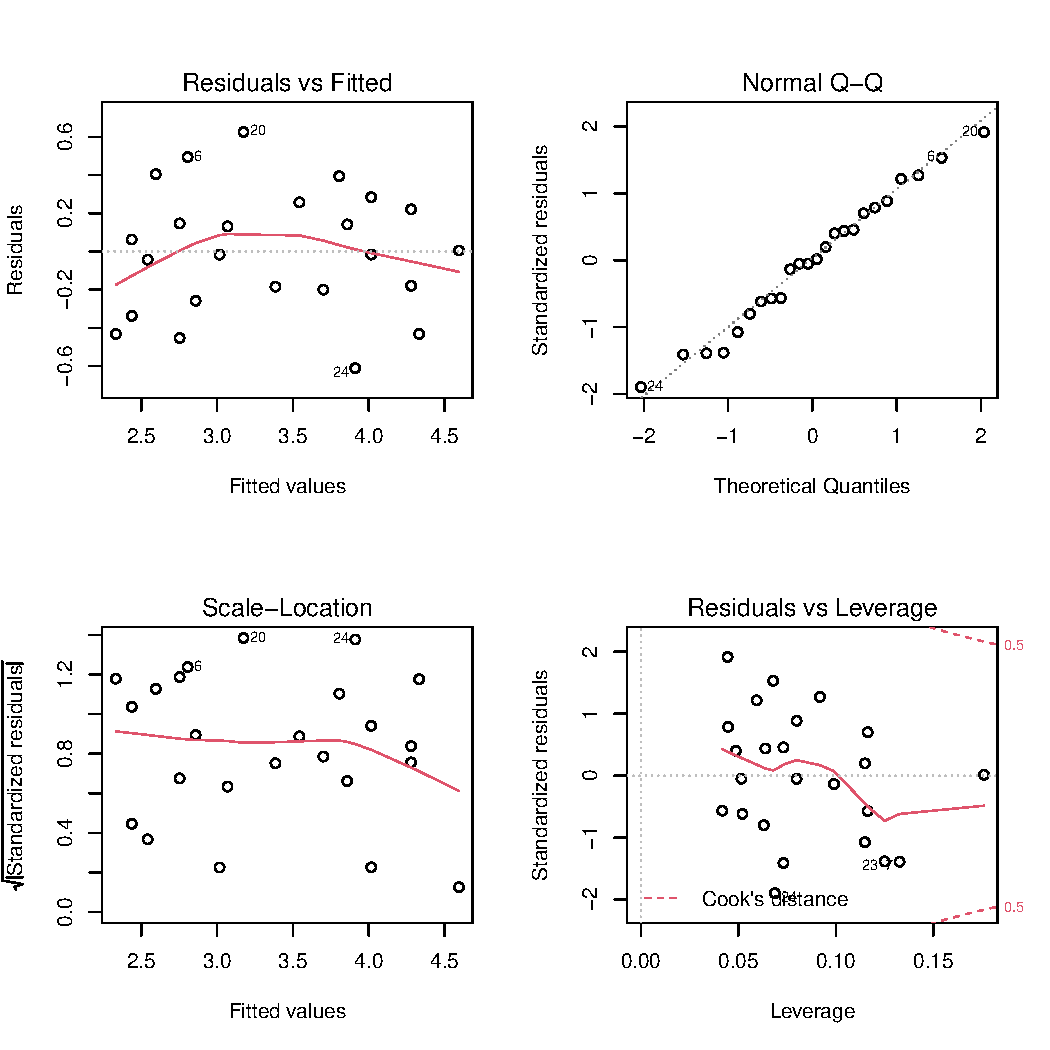
\includegraphics[width=1.0\textwidth]{part-b-fourplot.pdf}
    \caption{Διάγραμματα ελέγχου}
    \label{fig:part-b-fourplot}
\end{figure}

%%%%%%%%%%%%%%%%%%%%%%%%%%%%%%%%%%%%%%%%%%%%%%%%%%%%%%
%%%%%%%%%%%%%%%%%%%%%%%%%%%%%%%%%%%%%%%%%%%%%%%%%%%%%%
%%%%%%%%%%%%%%%%%%%%%%%%%%%%%%%%%%%%%%%%%%%%%%%%%%%%%%
%%%%%%%%%%%%%%%%%%%%%%%%%%%%%%%%%%%%%%%%%%%%%%%%%%%%%%
%%%%%%%%%%%%%%%%%%%%%%%%%%%%%%%%%%%%%%%%%%%%%%%%%%%%%%

\section{Μέρος}

\subsection{}
\subsubsection*{Εκφώνηση}
Να κατασκευαστεί ένα διάγραμμα διασποράς μεταξύ των δύο μεταβλητών \(y\) και \(x\) και να προσαρμοστεί ένα μοντέλο της μορφής \(y = 3 - a e^{\beta x}\).
\subsubsection*{Απάντηση}
Στα Σχήματα \ref{fig:part-c-scatter-original}, \ref{fig:part-c-scatter-transformed} και \ref{fig:part-c-scatter-transformed-detransformed} βλέπουμε τα σχετικά διαγράμματα διασποράς.
\begin{figure}[h]
    \centering
    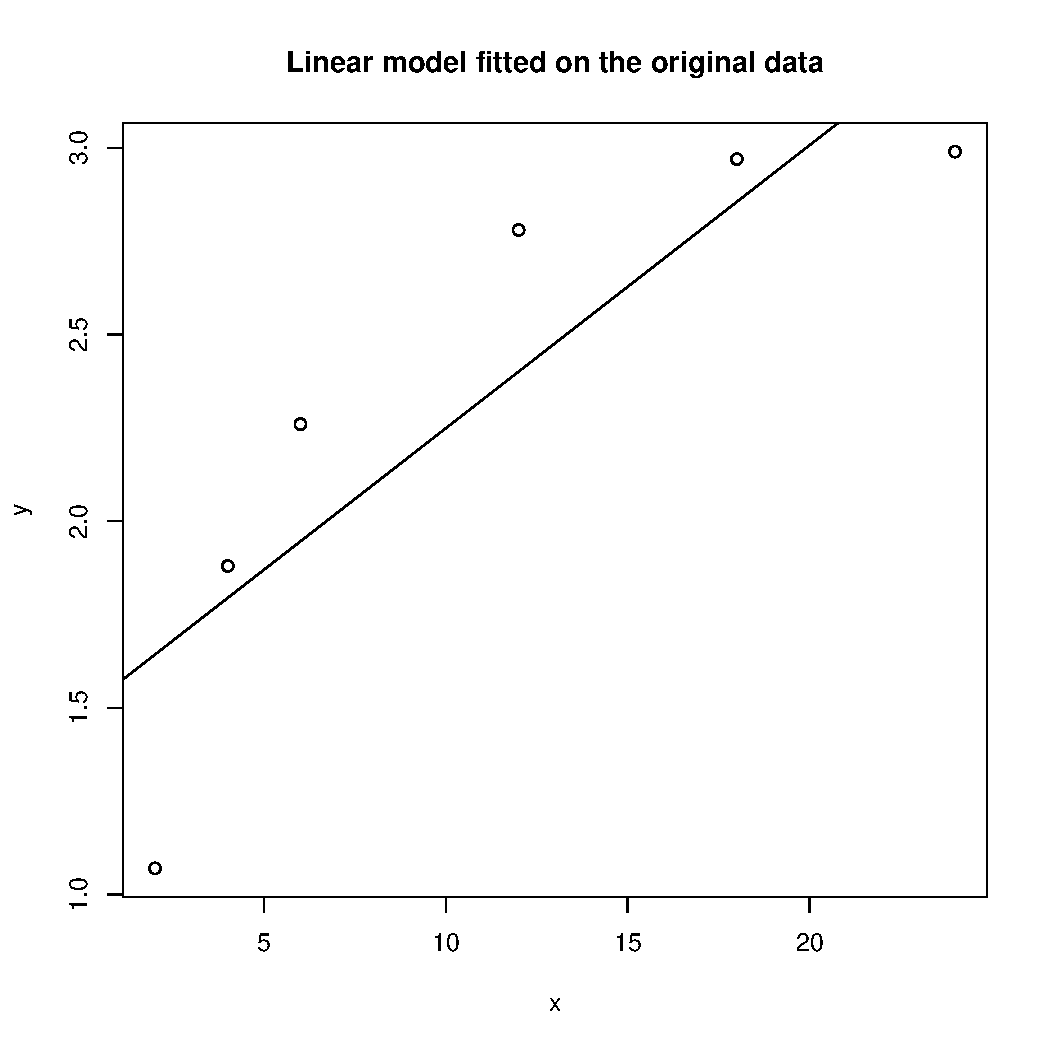
\includegraphics[width=1.0\textwidth]{part-c-scatter-original.pdf}
    \caption{Αρχικό διάγραμμα διασπορά, χωρίς μετασχηματισμό.}
    \label{fig:part-c-scatter-original}
\end{figure}
\begin{figure}[h]
    \centering
    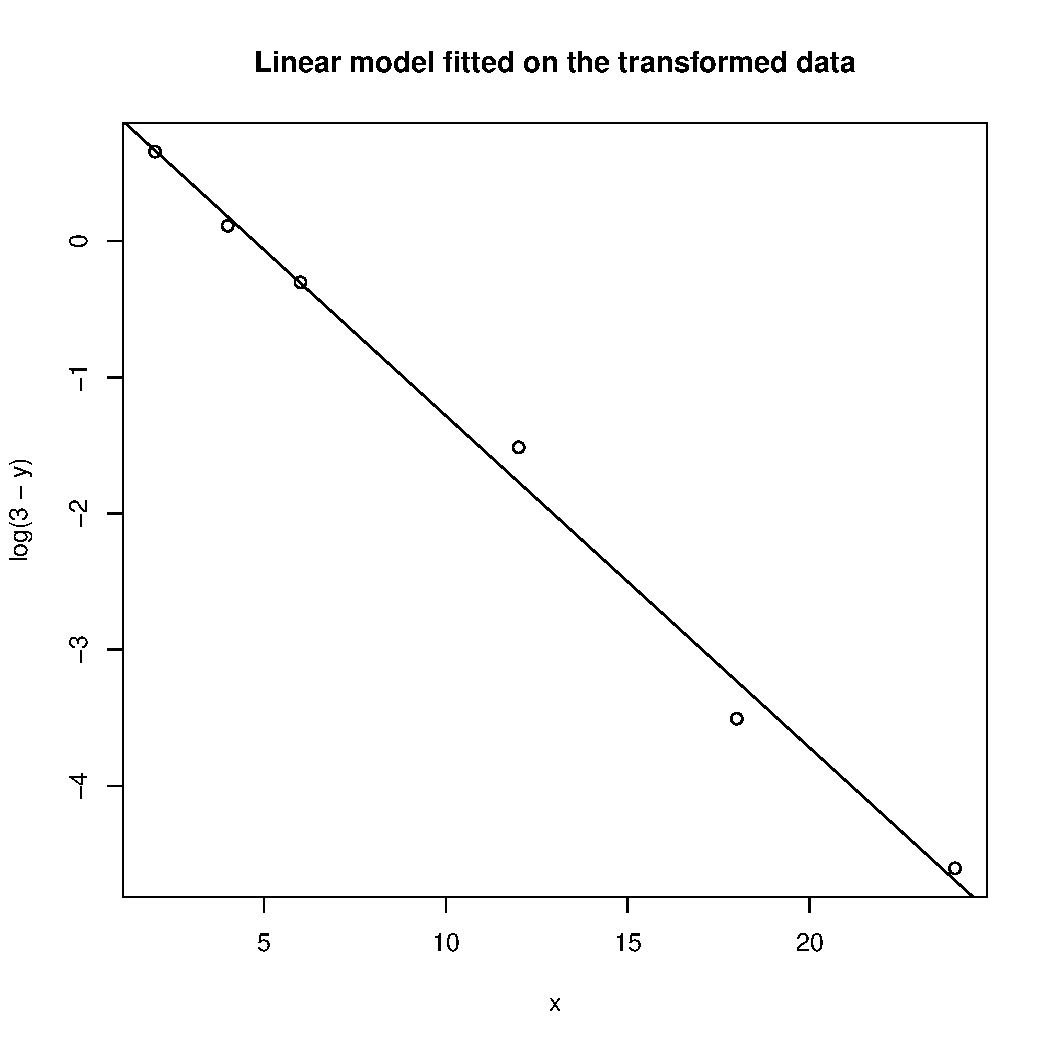
\includegraphics[width=1.0\textwidth]{part-c-scatter-transformed.pdf}
    \caption{Τελικό διάγραμμα διασποράς.}
    \label{fig:part-c-scatter-transformed}
\end{figure}
\begin{figure}[h]
    \centering
    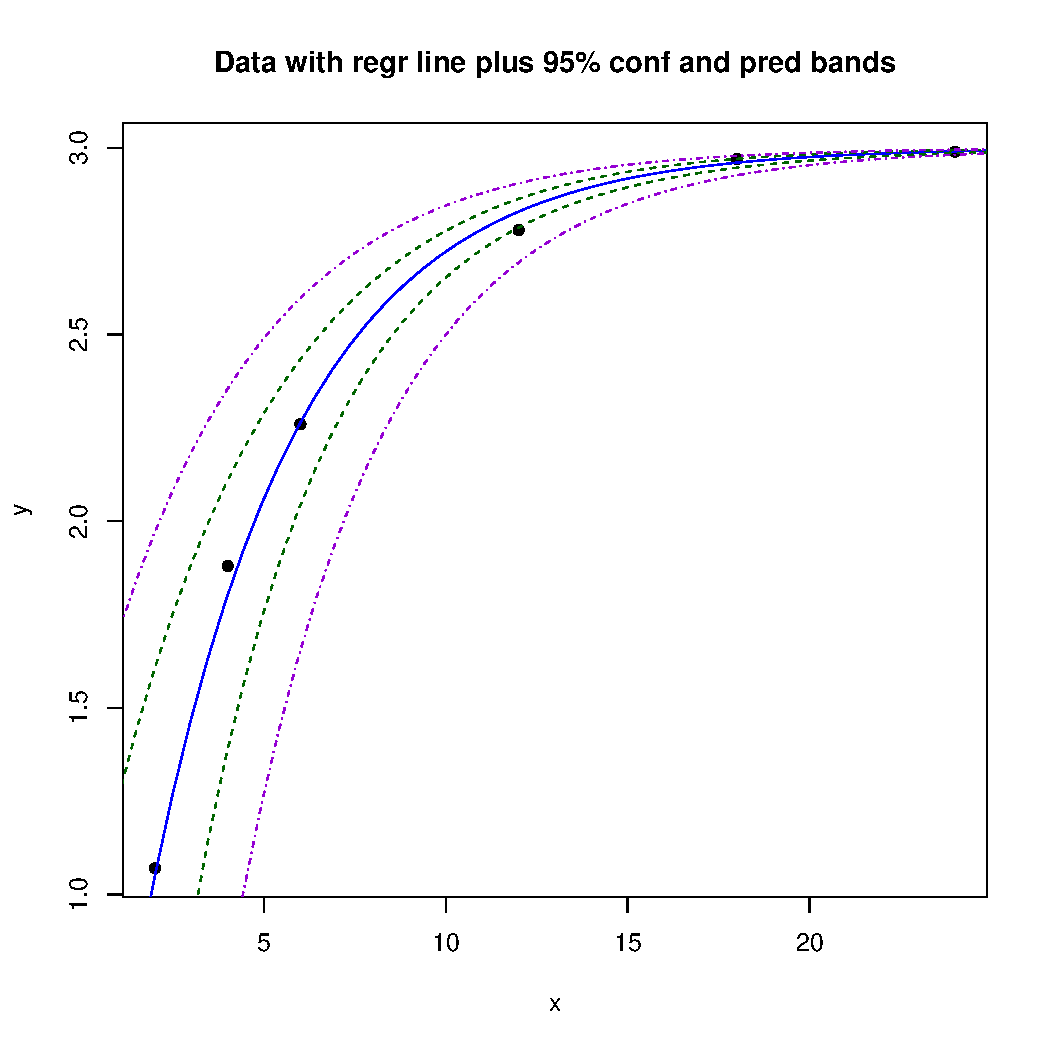
\includegraphics[width=1.0\textwidth]{part-c-scatter-transformed-detransformed.pdf}
    \caption{Τελικό διάγραμμα διασποράς, μετά από αντίστροφο μετασχηματισμό. Συμπεριλαμβάνονται διαστήματα πρόβλεψης και εμπιστοσύνης}
    \label{fig:part-c-scatter-transformed-detransformed}
\end{figure}


\subsection{}
\subsubsection*{Εκφώνηση}
Να εκτιμηθεί σημειακά η άγνωστη παρατήρηση \(y\) και να κατασκευαστεί ένα
95\% διάστημα εμπιστοσύνης (δ.ε.) για την πρόβλεψη της παρατήρησης \(y\),
καθώς και ένα προσεγγιστικό 95\% δ.ε. για τη μέση τιμή της, \(\E[y]\), όταν \(x = 9\).
\subsubsection*{Απάντηση}
Η εκτίμηση για το \(y\) είναι 2.646078.
Το 0.95-διάστημα πρόβλεψης για το \(y\) είναι το [2.361758, 2.803741].
Το 0.95-διάστημα εμπιστοσύνης για το \(\E[y]\) είναι το [2.555063 2.718475].
Στο σχήμα \ref{fig:part-c-scatter-transformed-detransformed} φαίνονται και οι "λωρίδες" πρόβλεψης και εμπιστοσύνης.

\end{document}


